\documentclass[a4paper,twoside,12pt]{book} 

\usepackage[xetex]{graphicx}
\usepackage{fontspec}
\usepackage{xunicode}
\defaultfontfeatures{Mapping=tex-text,Scale=MatchLowercase,Ligatures={Common}}
%\setmonofont{LMMonoLt10}
\setmainfont{Junicode}
\newICUfeature{LigType}{disc}{+dlig}

\usepackage{polyglossia}
\setdefaultlanguage{slovak}

\usepackage[
   backend=biber      % if we want unicode 
  ,style=iso-authoryear % iso-authoryear or iso-numeric for numeric citation method
%  ,style=authoryear-comp 
  ,babel=other        % to support multiple languages in bibliography
  %,sortlocale=cs_CZ   % locale of main language, it is for sorting
  ,bibencoding=UTF8   % this is necessary only if bibliography file is in different encoding than main document
]{biblatex}
\addbibresource{literatura.bib}

\usepackage[a4paper]{geometry}
\geometry{top=2.5cm,bottom=2.5cm,left=3.5cm,right=2.0cm}
\usepackage{setspace}
% \singlespacing
\onehalfspacing
\usepackage{changepage}
\usepackage{indentfirst}

\usepackage{url}
\usepackage[xetex]{hyperref}
     
% \usepackage{caption}
% \usepackage{subcaption}
\usepackage{subfig}
\usepackage{array}
  
%%definície konštánt a makier
\def \nazovUniverzity{Univerzita Komenského v Bratislave}
\def \NazovUniverzity{\textbf{\Large \sc \nazovUniverzity}} %\sc pre smallcaps
\def \nazovFakulty{Fakulta matematiky, fyziky a informatiky}
\def \NazovFakulty{\textbf{\large \sc \nazovFakulty}}
\def \nazovDiela{Vizualizácia algoritmov a dátových štruktúr}
\def \NazovDiela{\LARGE{\em \nazovDiela}}
\def \podnazovDiela{nie je}
\def \PodazovDiela{\large{\em \podnazovDiela}}
\def \typPrace{Bakalárska práca}
\def \TypPrace{\large{\typPrace}}
\def \autor{Viktor Tomkovič}
\def \veduci{Mgr. Jakub Kováč}
\def \rok{2012}
\def \miestoRok{Bratislava, \rok}
\def \cisloOdboru{2508}
\def \katedra{Katedra Informatiky FMFI}
\def \odbor{Informatika}
\def \program{Informatika}
\def\citet#1{\textcite{#1}}
\def\citep#1{\parencite{#1}}
%citat: argumenty sú citát a meno autora
\newcommand{\citat}[2]{\begin{flushright}\textsl{#1}\\#2\end{flushright}}
%strednp je vystredenie textu na nepárnej strane bez ohľadu na okraje(!!!), parametrom je text
\newcommand{\stredp}[1]{\begin{adjustwidth}{+0.50cm}{+0.00cm} \begin{center} #1 \end{center} \end{adjustwidth}}
%stredp je obdoba predošlého príkazu len pre párne strany
\newcommand{\strednp}[1]{\begin{adjustwidth}{+0.0cm}{+0.50cm} \begin{center} #1 \end{center} \end{adjustwidth}}
\def\todo#1{\par\smallskip{\scriptsize {\bf TODO: }#1}\par\smallskip}

\def\nul{\texttt{NULL}}
\def\makeset{$\mathop{\mathit{makeset}}(x)$}
\def\find{$\mathop{\mathit{find}}(x)$}
\def\union{$\mathop{\mathit{union}}(x, y)$}
\def\k{w}
%\def\kluc{kľúč}
\def\put{$\mathop{\mathit{insert}}(\k)$}
\def\find{$\mathop{\mathit{find}}(\k)$}
\def\delete{$\mathop{\mathit{delete}}(\k)$}
\def\trie{trie}
\def\uz{\hbox{\tt\$}}
\def\rank{\mathop{\mathit{rank}}}
\def\Java{\texttt{JAVA}}
 
\def\uv#1{„#1“}
\catcode`\"=\active \def "{\begingroup„\def "{\endgroup“}}
\begin{document}
\frontmatter
\pagestyle{plain}
\thispagestyle{empty}
\noindent
\strednp{
\NazovUniverzity\\ 
\NazovFakulty
}
\vfill
\strednp{
\NazovDiela
%% \centerline{\PodazovDiela}
\mbox{}\\
\bigskip
\TypPrace
}
\vfill
\strednp{\rok \hfill{\bf \autor}}
\newpage

\thispagestyle{empty}
\noindent
\strednp{\NazovUniverzity\\ \NazovFakulty}
\vfill
\strednp{\NazovDiela
%% \centerline{\PodazovDiela}
\mbox{}\\
\bigskip
\TypPrace
}
\vfill
\begin{tabular}{ l l }
\textbf{Študijný program:} & \program\\
\textbf{Študijný odbor:} & \cisloOdboru\ \odbor\\
\textbf{Školiace pracovisko:} & \katedra\\
\textbf{Vedúci práce:} &  \veduci
\end{tabular}
\bigskip\\
\bigskip\\
\bigskip\\
\bigskip\\
\strednp{\miestoRok \hfill{\bf \autor}}
\newpage

\noindent
~\vfill

\section*{Poďakovanie}
Veľká vďaka za to, že mi pomohli patrí môjmu školiteľovi Kubovi Kováčovi a 
mojim rodičom.\\
\bigskip\\
\newpage

\chapter*{Abstrakt}
Táto práca sa zaoberá vizualizáciou dátových štruktúr. Nadväzuje na bakalársku 
prácu Jakuba Kováča (2007) a rozvíja kompiláciu o ďalšie dátové štruktúry. V 
prvej časti sme tieto dátové štruktúry, konkrétne union-find, lexikografický 
strom a sufixový strom, definovali a konkrétne algoritmy popísali. V druhej 
časti sme spravili návrh aplikácie a popísali implementáciu. Práca je 
prehľadom dátových štruktúr s priloženým Java appletom na CD ako pomôckou pri 
vizualizácií.\\
Kľúčové slová: vizualizácia, ADŠ, algoritmy a dátové štruktúry, union-find, 
stringológia, lexikografický strom, trie, sufixový strom.

\newpage

\chapter*{Abstract}
This work is about visualization of algorithms and data structures. Continues 
the bachelor thesis of Jakub Kováč (2007) and extends the compilation by 
another data structures. In the first part are the structures, namely 
union-find, lexicographical tree (trie) and suffix tree, defined and the 
algorithms described. The second part is a description and a implementation of 
the software. The work is an overview of data structures with a software CD 
included.\\
Keywords: visualization, ADS, algorithms and data structures, union-find, 
stringology, loxicographical tree, trie, suffix tree.
\newpage

\mbox{}
\newpage

\tableofcontents\newpage
%\listoffigures
%\listoftables

\mainmatter
\pagestyle{headings}
\cleardoublepage
% \phantomsection
\addcontentsline{toc}{chapter}{Úvod}
\chapter*{Úvod}\label{chap:intro}

Dátové štruktúry a algoritmy tvoria základnú, prvotnú časť výučby 
informatiky. Vizualizácia algoritmov a dátových štruktúr je grafické 
znázornenie, ktoré abstrahuje od implementačných detailov a reprezentácie
v pamäti. Je teda vhodnou pomôckou pri výučbe i samoštúdiu. 

Ukážka nášho softvéru \emph{Gnarley Trees} je na obrázku~\ref{img:historia}.
Tento projekt začal ako bakalárska práca Jakuba Kováča \citep{kuko};
v tejto práci popisujeme nové dátové štruktúry, ktoré sme vizualizovali
a nové funkcie a vylepšenia, ktoré sme doplnili. Konkrétne ide o 
\emph{union-find problém}, \emph{písmenkový strom (trie)} a 
\emph{sufixový strom}. 

Softvér v súčasnosti vyvíja okrem Kuba Kováča aj Katka Kotrlová, ktorá 
vizualizovala rôzne typy háld a intervalové stromy, Táňa Tóthová, ktorá 
vizualizovala \emph{finger tree} a \emph{B$^+$-strom}.
Okrem vizualizácie softvér prerábame a neustále vylepšujeme.
Pavol Lukča ho doplnil o históriu krokov a operácií. Softvér je celý v 
slovenčine aj angličtine a je 
implementovaný v jazyku \Java. Dostupný je na stránke
{\url{http://people.ksp.sk/~kuko/gnarley-trees}} vo forme appletov
s jednotlivými dátovými štruktúrami, a tiež vo forme samostatného programu,
ktorý obsahuje všetky dátové štruktúry a je určený na používanie offline.

Našou snahou je vytvoriť kvalitný softvér nezávislý od operačného systému, 
ktorý bude vyhovovať ako pomôcka pri výučbe ako aj pri samoštúdiu a bude
voľne prístupný. 

%\bigskip
Predchádzajúci výskum v oblasti pedagogiky
zatiaľ nedokázal úplne preukázať pedagogickú efektívnosť
vizualizácií \citep{shaffer}, avšak viacero štúdií potvrdilo zvýšený záujem
a zapojenosť študentov \citep{naps02, hundhausen02}.

Rozmach vizualizácie algoritmov priniesla najmä \Java\ a jej fungovanie 
bez viazanosti na konkrétny operačný systém. Kvalita iných existujúcich 
vizualizácií sa líši a keďže ide o ľahko naprogramovateľné programy, je ich 
veľa a sú pomerne nekvalitné \citep{shaffer}. 
Zbieraním a analyzovaním kvality sa venuje skupina AlgoViz (\hbox{\url{http://algoviz.org/}}).

Zaujímavé je pozorovanie, že určovanie si vlastného tempa pri vizualizácií 
je veľká pomôcka. Naopak, ukazovanie pseudokódu alebo nemožnosť určenia si
vlastného tempa (napríklad animácia bez možnosti pozastavenia), takmer 
žiadne zlepšenie neprináša \citep{shaffer,saraiya}.

%\bigskip
% Zvyšok článku je organizovaný nasledovne: V sekcií 2 popisujeme implementované
% vylepšenia týkajúce sa vizualizácie, grafiky a ovládania, v sekciách 3 až 6
% nové dátové štruktúry, ktoré sme implementovali a vizualizovali: vyvážené
% stromy, haldy, union-find a písmenkové stromy.

Prácu sme rozdelili na popis jednotlivých dátových štruktúr, ktoré sme 
vizualizovali a popis samotného softvéru. V kapitolách~
\ref{chap:uf}, \ref{chap:trie} a \ref{chap:sx} je postupne popis 
\emph{union-find}, \emph{písmenkového stromu} a \emph{sufixového stromu}. 
V~kapitole~\ref{chap:popis} je popis softvéru a 
v~kapitole~\ref{chap:implementacia} je implementácia.
 
\begin{figure}
\centering
\greybox{%
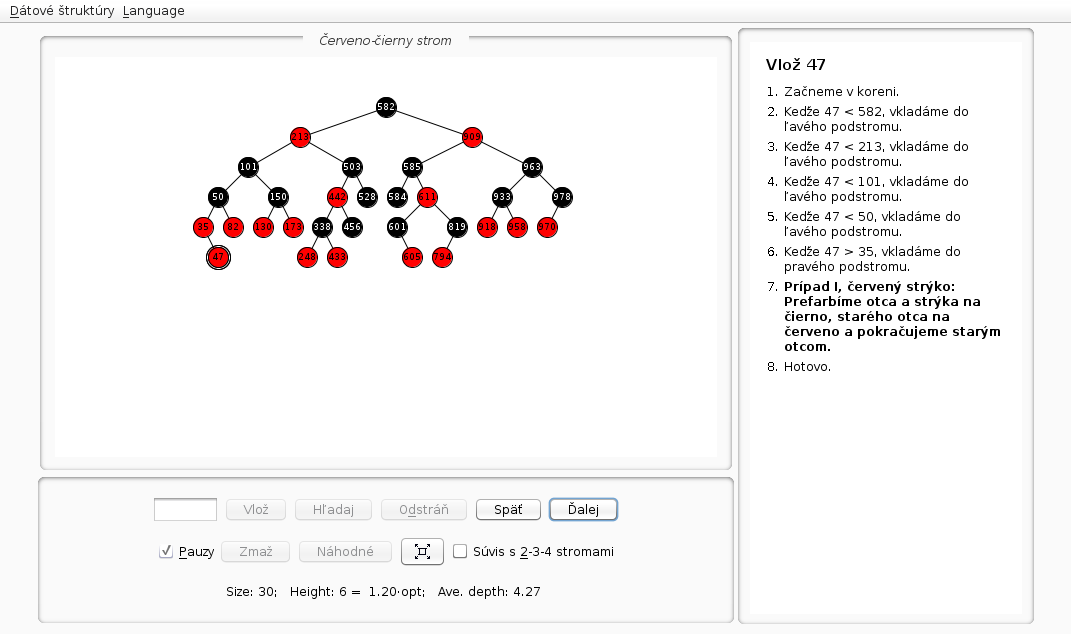
\includegraphics[width=\columnwidth]{obrazky/gt.png}%
}
\caption{\emph{Softvér Gnarley Trees.} V ovládacom paneli dole môže používateľ
zvoliť operáciu a vstupnú hodnotu a sledovať priebeh algoritmu (zobrazené je vkladanie
prvku 47). Používateľ postupuje vlastným tempom  pomocou tlačidiel \uv{Ďalej} alebo
\uv{Späť}. Vpravo je popis vykonávaných krokov; kliknutím na konkrétny krok v histórií
sa môže používateľ vrátiť.}
\label{img:historia} 
\end{figure}

\chapter{Union-find problém}\label{chap:uf}

V niektorých aplikáciach potrebujeme udržiavať prvky rozdelené do skupín
(disjunktných množín), pričom skupiny sa môžu zlučovať a my potrebujeme
pre daný prvok efektívne zistiť, do ktorej skupiny patrí. Predpokladáme,
že každá množina $S$ je jednoznačne určená jedným svojim zástupcom $x\in S$
a potrebujeme implementovať nasledovné tri operácie:

\begin{itemize}
\item $\makeset(x)$ -- vytvorí novú množinu $S=\{x\}$ s jedným prvkom; %,
                   %ktorý nepatrí do žiadnej inej množiny;
\item $\union(x, y)$ -- ak $x, y$ sú zástupcovia množín $S$ a $T$,
                 $\union$ vytvorí novú množinu $S\cup T$,
                 pričom $S$ aj $T$ zmaže. Zástupcom novej množiny $S\cup T$
                 je $x$ alebo $y$;
\item $\find(x)$ -- nájde zástupcu množiny, v ktorej sa 
                prvok $x$ nachádza.
\end{itemize}
 
\section{Použitie}\label{sec:uf-pouzitie}

Union-find sa dá použiť na reprezentáciu neorientovaného grafu,
do ktorého pridávame hrany a odpovedáme na otázku: "Sú dané dva
vrcholy spojené nejakou cestou?" (t.j.\ sú v~rovnakom komponente súvislosti?)
Medzi najznámejšie aplikácie patria Kruskalov algoritmus na nájdenie najlacnejšej
kostry \citep{kruskal} a unifikácia \citep{unif}.

\citet{cholesky} ukázali, ako sa dá union-find použiť pri Choleského dekompozícií
riedkych matíc. Autori navrhli efektívny algoritmus, ktorý zistí počet nenulových
prvkov v každom riadku a stĺpci výslednej matice, čo slúži na efektívnu alokáciu
pamäte.

Pre offline verziu úlohy, kde sú všetky operácie dopredu známe, \citet{offline-uf}
navrhli lineárny algoritmus. Článok obsahuje tiež viacero aplikácií v teoretickej
informatike.

\section{Popis}
Dátová štruktúra \emph{union-find} sa reprezentuje ako les, kde každý strom zodpovedá
jednej množine a korene stromov sú zástupcovia množín. Pri implementácií si
stačí pre každý prvok $x$ udržiavať smerník $p(x)$ na jeho otca
(pre koreň je $p(x)=\nul$).

\paragraph{Vytváranie prvkov.}%
Operácia $\makeset(x)$ teda vytvorí nový prvok $x$ a nastaví $p(x) = \nul$. 

\paragraph{Hľadanie zástupcu.}%
Operáciu $\find(x)$ vykonáme tak, že budeme sledovať cestu po smerníkoch, až 
kým nenájdeme zástupcu. 

\paragraph{Spájanie množín.}%
Operáciu $\union(x, y)$ najjednoduchšie vykonáme tak, že presmerujeme smerník 
$p(y)$ na prvok $x$, teda $p(y) \gets x$. 
Môžeme ľahko pozorovať, že takýto \emph{naivný} spôsob je neefektívny, 
lebo nám operácia $\find(x)$ v najhoršom prípade na $n$ prvkoch trvá $\Omega(n)$ 
krokov. 

\bigskip
Existujú dva prístupy ako zlepšiť operácie a tým aj zrýchliť ich vykonanie. 
Sú to: heuristika \emph{spájanie podľa ranku} a rôzne heuristiky na 
\emph{kompresiu cesty}. 

\section{Heuristika na spájanie}\label{sec:komp-union}

Prvá heuristika pre každý vrchol $x$ udržuje hodnotu $\rank(x)$,
ktorá určuje najväčšiu možnú hĺbku podstromu s koreňom $x$.
Pri o\-pe\-rá\-cií $\makeset(x)$ zadefinujeme $\rank(x) = 1$. 
Pri o\-pe\-rá\-cií $\union(x, y)$ porovnáme $\rank(x)$ a $\rank(y)$
a vždy napojíme strom s menším rankom pod strom s väčším rankom.
Ak majú oba stromy rovnaký rank, napojíme povedzme $x$ pod $y$
a $\rank(y)$ zvýšime o 1.
%aby sme zistili, ktorý zástupca predstavuje menší strom. 
% Smerník tohto zástupcu potom napojíme 
% na zástupcu s výšším rankom. Zástupca novej množiny bude ten s vyšším rankom. 
% Ak sú oba ranky rovnaké, vyberieme ľubovoľného zo zástupcov $x$ a $y$, 
% jeho rank zvýšime o jeden a smerník ostatného zástupcu bude ukazovať 
% na tohto zástupcu. %Zástupcom novej množiny bude vybratý zástupca. 

\section{Heuristiky na kompresiu cesty}\label{sec:komp-cesta}
      
\begin{figure}
\centering
\subfloat[Pred vykonaním kompresie.]{
\label{img:komp1}
% ,width=0.4\textwidth
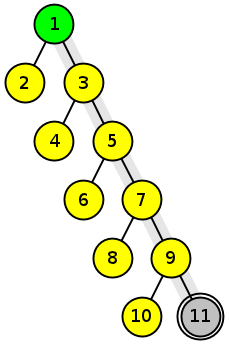
\includegraphics[height=0.24\textheight]{obrazky/komp1.png}
}
\qquad
\subfloat[Úplná kompresia.]{
\label{img:komp2}
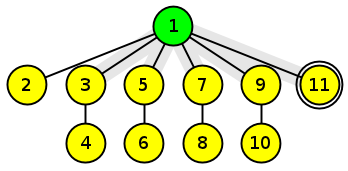
\includegraphics[height=0.12\textheight]{obrazky/komp2.png}
}

\subfloat[Delenie cesty.]{
\label{img:komp3}
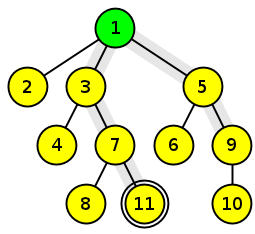
\includegraphics[height=0.16\textheight]{obrazky/komp3.png}
}
\qquad
\subfloat[Pólenie cesty.]{
\label{img:komp4}
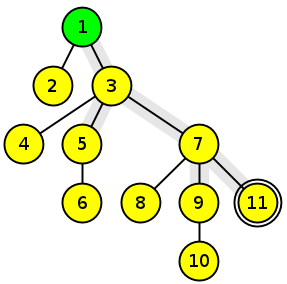
\includegraphics[height=0.20\textheight]{obrazky/komp4.png}
}
\caption{\emph{Kompresia cesty z vrcholu 11 do koreňa.} 
Cesta je vyznačená šedou. 
Pri úplnej kompresii~\subref{img:komp2} sa všetky vrcholy 
napoja na zástupcu. Pri delení cesty~\subref{img:komp3} a pólení 
cesty~\subref{img:komp4} sa cesta skráti približne na polovicu.}
\label{img:kompresia}
\end{figure}
 
Druhou heuristikou je kompresia cesty. Algoritmov na efektívnu kompresiu 
cesty je veľa \citep{paths2}, tu popíšeme tie najefektívnejšie. Prvou z nich 
je \emph{úplná kompresia} \citep{comp1}. Pri vykonávaní operácie $\find(x)$, po 
tom, ako nájdeme zástupcu, napojíme všetky vrcholy po ceste priamo pod koreň 
(obr.~\ref{img:komp2}). Toto síce trochu spomalí prvé hľadanie, ale výrazne 
zrýchli ďalšie hľadania pre všetky prvky na ceste ku koreňu. Druhou 
heuristikou je \emph{delenie cesty} \citep{comp2}. Pri vykonávaní operácie 
$\find(x)$ pripojíme každý vrchol v ceste od vrcholu $x$ po koreň stromu na otca 
jeho otca (obr.~\ref{img:komp3}). Treťou heuristikou je \emph{pólenie cesty} 
\citep{comp2}. Pri vykonávaní operácie $\find(x)$  pripojíme každý druhý vrchol 
v ceste od vrcholu $x$ po koreň stromu na otca jeho otca 
(obr.~\ref{img:komp4}).

Časová zložitosť union-findu záleží od toho, koľko prvkov je v množinách a koľko je 
operácií celkovo vykonaných operácií. Všetky uvedené spôsoby ako vykonať 
operáciu $\find(x)$ sa dajú použiť s obomi realizáciami operácie $\union$. 
Počet prvkov označme $n$ a počet operácií $m$. V praxi je zvyčajne počet 
operácií oveľa väčší ako počet prvkov. Pri tomto predpoklade ($m\geq n$) je 
pri použití spájania podľa ranku časová zložitosť pre algoritmus bez kompresie 
$\Theta(m\log n)$ a pre všetky tri uvedené typy kompresií 
$\Theta(m\mathop{\alpha}(m,n))$, kde $\alpha$ je inverzná Ackermannova funkcia 
tak, ako ju definoval Tarjan \citep{dsna}. 
V tabuľke~\ref{fig:uf:comp} je porovnanie časových zložitostí \citep{paths2}.

\begin{table}
\centering
\small
%\footnotesize %toto tu mám nechať?
\subfloat[Časová zložitosť pre union-find, keď $m \geq n$.][Prehľad časových zložitostí, ak $m \geq n$.]{
\begin{tabular}{m{5cm}m{4cm}m{4cm}}
& Naivné spájanie & Spájanie podľa ranku \tabularnewline
\hline
Naivné hľadanie & $\Theta\left( mn\right)$ & $\Theta\left( m\log n\right)$ \tabularnewline
Úplná kompresia, delenie cesty, pólenie cesty & $\Theta\left(m\log _{1+m/n} n \right)$ & $\Theta\left( m\alpha\left( m, n\right) \right)$ \tabularnewline
\label{fig:uf:comp1}
\end{tabular}
}
\qquad
\subfloat[Časová zložitosť pre union-find, keď $m < n$.][Prehľad časových zložitostí, ak $m < n$.]{
\begin{tabular}{m{5cm}m{4cm}m{4cm}}
& Naivné spájanie & Spájanie podľa ranku \tabularnewline
\hline
Naivné hľadanie & $\Theta\left( mn\right)$ & $\Theta\left(n + m\log n\right)$ \tabularnewline
Úplná kompresia& $\Theta\left(n + m\log  n \right)$ & $\Theta\left(n + m\alpha\left( n, n\right) \right)$ \tabularnewline
Delenie cesty & $\Theta\left(n \log m \right)$ & $\Theta\left(n + m\alpha\left( n, n\right) \right)$ \tabularnewline
Pólenie cesty & $\Omega\left(n + m\log n \right)$, $O\left(n\log m\right)$ & $\Theta\left(n + m\alpha\left( n, n\right) \right)$ \tabularnewline
\label{fig:uf:comp2}
\end{tabular}}
\caption{\emph{Porovnanie časových zložitostí pre rôzne kombinácie hľadaní prvkov a 
spájaní množín pre union-find \citep{paths2}.} Počet prvkov je $n$ a počet operácií je $m$. 
Inverzná Ackermannova funkcia je označená ako $\alpha$. V praxi zväčša platí, že $m > n$.}
\label{fig:uf:comp}
\end{table}

% \section{Vizualizácia}
% Dátovú štruktúru union-find sme vizualizovali ako les. Pre názorné 
% oddelenie množín sme si zvolili pravidlo, ktoré zakazovalo vykresliť vrchol 
% z iného stromu (prvok inej množiny) 
% napravo od najľavejšieho vrcholu a naľavo od napravejšieho vrcholu inej 
% množiny. Jednotlivé množiny sme už vykreslovali tesným Walkerovým algoritmom 
% \citep{walker}. Vizualizácia poskytuje všetky vyššie spomínané heuristiky a 
% aj tlačidlo na vykonanie viacerých náhodných spojení naraz. Toto je užitočné, 
% keď chce uživateľ vidieť, ako dátová štruktúra vyzerá, po vykonaní 
% veľa operácií.
% 



\chapter{Písmenkový strom}\label{chap:trie}

\emph{Písmenkový strom} reprezentuje množinu slov. Oproti binárnym 
vyhľadávacím stromom je hlavný rozdiel v tom, že kľúče nie sú uložené 
vo vrcholoch, ale samotná poloha v strome určuje kľúč (slovo). 

\section{Popis}\label{sec:trie:popis}
Písmenkový strom je \emph{zakorenený strom}, v~ktorom každá hrana obsahuje 
práve jeden znak z abecedy alebo \emph{ukončovací znak}. Teda, každá cesta 
z koreňa do listu so znakmi $w_1, w_2, \ldots, w_n, \uz$ prirodzene 
zodpovedá slovu $w=w_1w_2\cdots w_n$. \emph{Ukončovací znak} je ľubovoľný, 
dopredu dohodnutý symbol, ktorý sa v abecede nenachádza (napr. \uz). 

Písmenkový strom je \emph{asociatívne pole (slovník)}, čiže 
poskytuje tieto tri operácie:
\begin{itemize}
\item $\put(\k)$ -- pridá do stromu slovo $\k$;
\item $\find(\k)$ -- zistí, či sa v strome slovo $\k$ nachádza;
\item $\delete(\k)$ -- odstráni zo stromu slovo $\k$.
\end{itemize}
Všetky operácie začínajú v koreni a ku slovu pridávajú ukončovací znak, 
teda pracujú s reťazcom $\k\uz$. 

\paragraph{Vkladanie slova.}%
Operácia $\put(\k)$ vloží do stromu vstupný reťazec tak, že z reťazca číta znaky 
a prechádza po príslušných hranách. Ak hrana s daným symbolom neexistuje, 
pridá ju (pozri obr.~\ref{img:trieinsert}).

\begin{figure}
\centering
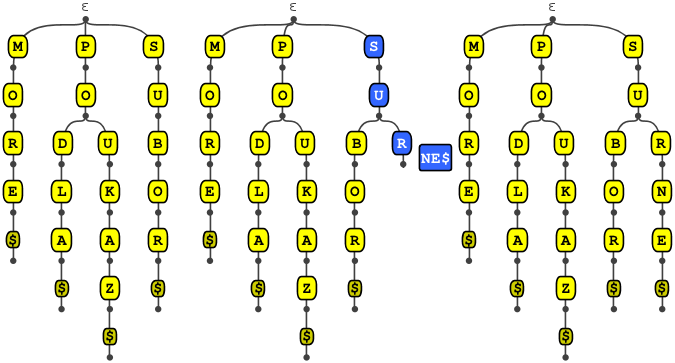
\includegraphics[width=0.9\columnwidth]{obrazky/trieinsertsmall.png}
\caption{\emph{Vloženie slova \uv{{\tt SURNE}}.} Začiatok slova 
\uv{{\tt SU}} sa v strome nachádza, ešte treba pripojiť hrany 
so znakmi {\tt R}, {\tt N}, {\tt E} a \uz.} 
\label{img:trieinsert} 
\end{figure}

\paragraph{Hľadanie slova.}%
Operácia $\find(\k)$ sa spustí z koreňa podľa postupnosti znakov. Ak hrana, 
po ktorej sa má spustiť neexistuje, dané slovo sa v strome nenachádza. 
Ak prečíta celý vstupný reťazec, dané slovo sa v strome nachádza.

\paragraph{Mazanie slova.}%
Operácia $\delete(\k)$ najprv pomocou operácie $\find(\k)$ zistí umiestnenie slova. 
Ak sa slovo v strome nachádza, algoritmus odstráni hranu s ukončovacím 
znakom a vrchol, ktorý bol na nej zavesený. V tomto štádiu sa nám môže 
stať, že v strome ostane \emph{mŕtva vetva} -- nie je ukončená 
ukončovacím znakom. Pre fungovanie stromu to nevadí, všetky operácie by 
prebiehali správne, ale takto štruktúra zaberá zbytočne veľa miesta. 
Preto je dobré túto mŕtvu vetvu odstrániť (pozri obr.~\ref{img:triedelete}).

\begin{figure}
\centering
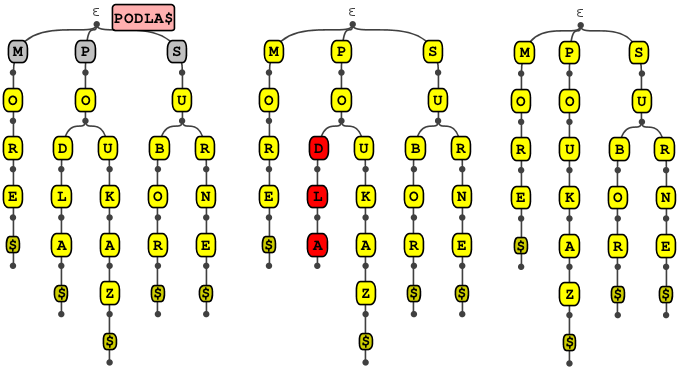
\includegraphics[width=0.9\columnwidth]{obrazky/triedeletesmall.png}
\caption{\emph{Odstránenie slova \uv{{\tt PODLA}}.} Po odstránení 
\uz\ nám v strome ostane nepotrebá prípona \uv{{\tt DLA}} (mŕtva vetva), 
ktorá je vyznačená červenou.}
\label{img:triedelete} 
\end{figure}

Všetky tri operácie majú časovú 
zložitosť $O(|\k|)$, kde $|\k|$ je dĺžka slova.

\section{Použitie}\label{sec:trie:pouzitie}
Prvýkrát navrhol písmenkový strom \citet{fredkin}, ktorý používal názov 
\emph{trie memory}\footnote{Z anglického re\emph{trie}val -- získanie.}, 
keďže išlo o spôsob udržiavania dát v pamäti. 
\citet{patricia} navrhol písmenkový strom, v ktorom sa každá cesta bez vetvení
skomprimuje do jedinej hrany (na hranách potom nie sú znaky, ale slová).
Táto štruktúra je známa pod menom \emph{PATRICIA} (tiež \emph{radix tree},
resp.\ \emph{radix trie}) a využíva sa napríklad v \emph{routovacích tabuľkách}
\citep{radix}.

Písmenkový strom (tzv.\ \emph{packed trie} alebo \emph{hash trie}) sa používa
napríklad v programe \TeX\ na slabikovanie slov \citep{liang}.
Pôvodný návrh \citep{fredkin} ako uložiť \trie\ do pamäte zaberal
príliš veľa nevyužitého priestoru. \citet{liang} však navrhol, ako
tieto nároky zmenšiť.

Písmenkové stromy sa podobajú na \emph{konečné automaty}. 
Vznikli rôzne modifikácie stromov na automaty, ktorých hlavnou výhodou je, 
že v komprimovanej podobe spájajú nielen predpony, ale aj prípony slov 
a teda v slovách ľudských jazykov výrazne znižujú pamäťový priestor potrebný 
na uchovanie dátovej štruktúry. Vďaka tomu sa využívajú na jazykovú korekciu, 
automatické dopĺňanie slov a podobne \citep{scrabble,ca}. 

Ďalšie použitie písmenkového stromu je pri triedení zoznamu slov. 
Všetky slová sa pridajú do stromu a potom sa spraví \emph{preorderový prechod} 
stromu. Túto myšlienku spracovali \citet{burstsort1} a veľmi výrazne zrýchlil 
triedenie dlhých zoznamov slov. Neskôr tento algoritmus vylepšili 
\citet{burstsort2}. Kvôli tomu, ako algoritmus pracuje, 
sa nazýva \emph{burstsort}.

% Špeciálnym použitím písmenkového stromu je vytvorenie stromu zo všetkých 
% prípon slova. Táto dátova štruktúra sa nazýva \emph{sufixový strom} a dá sa 
% mo\-di\-fi\-ko\-vať na udržiavanie viacerých slov. Tieto štruktúry majú 
% veľmi veľa praktických využití \citep{gusfield}. 

% \section{Vizualizácia} 
% Pri vizualizácií písmenkového stromu sme použili 
% Walkerov algoritumus pre úsporné rozloženie vrcholov v strome
% \citep{walker}. Keď má vrchol viacej synov a hrany kreslíme priamo, tak vzniká 
% nedostatok priestoru pre umiestnenie znakov na hrany. Preto sme sa rozhodli 
% kresliť hrany zakrivene, podľa Bézierovej krivky určenej štyrmi bodmi. 
% Vo vizualizácií sa dajú vložiť náhodné slová podľa momentálne nastaveného 
% jazyka. Taktiež sa automaticky odstraňuje diakritika a interpunkcia, takže 
% sa dá naraz vložiť súvislý text.


\chapter{Sufixový strom}\label{chap:sx}

\emph{Sufixový strom} je písmenkový strom pre všetky \emph{sufixy (prípony)} 
daného slova. Jeho veľká výhoda spočíva v rýchlom zostrojení a veľkom množstve 
efektívnych algoritmov na ňom. V softvéri sme vizualizovali jeho zostrojenie, a 
preto ho aj tu popíšeme.

\section{Zostrojenie sufixového stromu}
Existuje veľa spôsobov ako zotrojiť sufixový strom. Najjednoduchšie riešenie 
je využiť písmenkový strom a pridať do neho všetky sufixy. Takéto riešenie má 
časovú aj pamäťovú zložitosť $O(n^2)$. 

\citet{ukkonen} navrhol, ako zostrojiť strom rýchlejšie a za behu. 

\section{Ukkonenov algoritmus}

Hlavnou myšlienkou algoritmu je pre slovo $w_1w_2w_3\cdots w_n\uz$ postupne 
vytvoriť suffixové stromy pre slová $w_1, w_1w_2,\ldots, 
w_1w_2w_3\cdots w_n\uz$. Označme tieto stromy $T(1), T(2),\ldots, T(n), T$. 
Teda, vytvárame $n$ stromov a každý zatiaľ na vytvorenie potrebuje $O(n^2)$ 
krokov. Toto je na prvý pohľad veľmi nešikovné riešenie pretože počet 
krokov potrebných na zostrojenie všetkých stromov je $O(n^3)$. 
Avšak zopár vylepšeniami je možné tento algoritmus zrýchliť až na hranicu 
$O(n)$ a to aj pre rýchlosť, aj pre pamäť. 

% well, nikde nie je napísané, že je to theta, ale hádam potrebujeme aspoň 
% prečítať vstup, nie?

Môžeme si všimnúť, že keď už máme vytvorený strom 
$T(i-1)$ (ktorý obsahuje sufixy $w_1\cdots w_{i-1}, w_2\cdots w_{i-1}, \ldots, 
w_{i-1}$), tak pre vytvorenie stromu $T(i)$ netreba znovu vytvárať nový strom 
a pridávať do neho sufixy $w_1\cdots w_{i-1}w_i, w_2\cdots w_{i-1}w_i, \ldots, 
w_{i-1}w_i$, ale stačí rozšíriť existujúce sufixy o znak $w_i$.

Druhým dobrým pozorovaním je fakt, že keď máme znak $a$, slovo $v$ 
a v strome sa nachádza sufix $a v$, tak sa v strome určite 
nachádza aj slovo $v$. Vyplýva to zo základnej vlastnosti sufixových stromov 
--  sufixový strom obsahuje všetky sufixy.
 
\subsection{Sufixové linky}

Pri vytváraní stromu $T(i)$ zo stromu $T(i-1)$ postupne rozširujeme sufixy, no 
bolo by neefektívne ich vždy vyhľadávať z koreňa. Preto zavedieme 
\emph{sufixový link} pre každý vrchol okrem koreňa, ten sufixový link nemá. 
Pre vrchol končiaci sufix $av$ to je vrchol končiaci sufix $v$. 

Algoritmus teda zmeníme tak, že namiesto opätovného vyhľadávania sufixu z 
koreňa, vyhľadáme bod, z ktorého začneme pridávať len raz a ďalej sa 
navigujeme po linkoch. Po pridaní vrchola, nazvime ho $u_i$, do stromu 
prejdeme sufixovým linkom na miesto, kde opäť pripojíme vrchol $u_{i+1}$. 
Vytvoríme sufixový link pre vrchol $u_i$ -- bude to smerník na $u_{i+1}$. 

Ako nám to pomohlo zlepšiť časovú zložitosť? Teraz nám stačí pre každý z 
$n$ stromov nájsť sufix, kde začneme rozširovať strom. Ten nájdeme na $O(n)$ 
krokov. Rozšírienie stromu o jeden znak zaberie tiež $O(n)$ krokov. Dokopy 
venujeme jednému stromu $O(n)$ krokov a $n$ stromom venujeme $O(n^2)$.

Ďalším zlepšením bude pamäťová optimalizácia.

\subsection{Zníženie nárokov na pamäť}

Veľmi priamočiarym krokom k zlepšeniu pamäťovej náročnosti sa zdá byť 
kompresia hrán. Po nej na hranách 
nie je len jeden znak, ale celý reťazec znakov. Takto má celý strom dovedna 
$O(n)$ hrán. Dôvod, prečo ju uvádzam až tu, je jednoduchý. 
Prichádza prirodzene s druhým vylepšením. Namiesto toho, aby sme si na hrane 
pamätali celý reťazec, budeme si na nej pamätať len počiatočnú a konečnú 
pozíciu v slove, pre ktorý beží algoritmus\footnote{Tento krok predpokladá, 
že vieme adresovať reťazec priamo.}. Po týchto zlepšeniach nám stačí 
pamätať si $O(n)$ informácií. 

Keďže kompresiou sa niektoré vrcholy stratili, musíme upraviť spôsob, ako sa 
pohybovať po sufixových linkoch. Úprava bude mierna. Po pridaní znaku 
prejdeme do najbližšieho vrcholu a popri tom si zapamätáme reťazec znakov, 
ktorý sme prešli. Keďže si znaky na hrane pamätáme ako dvojicu čísel, toto 
nám zaberie len $O(1)$ krokov. Keď následne prejdeme po sufixovom linku, 
vyhľadáme zapamätaný reťazec. Z vlastností stromu vyplýva, že stačí 
pozerať len na prvé písmeno každej hrany preto, aby sme vedeli, či po nej 
máme prejsť alebo nie.

To, akým spôsobom sa písmenko po vyhľadaní pridá a kde vieme ušetriť počet 
krokov, popíšeme v nasledujúcej časti.

\subsection{Rozširovanie stromu}

Pri rozširovaní stromu o písmenko môžu nastať tieto tri prípady:
\begin{itemize}
\item \emph{prvý prípad:} písmenko pripájame k vrcholu, z ktorého nepokračuje 
hrana, a teda je listom;
\item \emph{druhý prípad:} písmenko pripájame na miesto, z ktorého nepokračuje 
hrana s daným písmenkom, ale pokračuje z neho hrana s iným písmenkom;
\item \emph{tretí prípad:} písmenko pripájame na miesto, z ktorého pokračuje 
hrana s daným písmenkom.
\end{itemize}

Po tomto rozdelení môžeme ľahšie pozorovať ďalšie veci. Prvou je, že akonáhle 
vytvoríme novú vetvu (nastane prvý alebo druhý prípad), tak ju v ďalších 
krokoch môžeme len rozšíriť. Čiže, ak sme raz pridali list, ten aj listom 
navždy ostane. Túto skutočnosť môžeme využiť v implementácií tak, že pri 
vytváraní hrany 
nastavíme indexy hrany na $i$ (index momentálneho písmenka, o ktoré strom 
rozširujeme) a $e$, čo je globálna premenná označujúca momentálny koniec v 
slove, ktorá sa každým rozšírením zvýši o jeden.

Druhým pozorovaním je, že po prvom výskyte tretieho prípadu sa strom už 
nerozšíri. Vyplýva to zo základnej vlastnosti sufixového stromu: ak 
rozširujeme strom o písmenko $w_i$ a v strome je slovo $w_j\cdots w_i$, tak 
sú v ňom aj slová $w_{j+1}\cdots w_i, w_{j+2}\cdots w_i, \ldots, w_i$.

Ďalším pozorovaním je, že pri rozširovaní najprv nastávajú prvé prípady, 
potom druhé a až potom tretie.

So všetkými týmito poznatkami môžeme konečne skonštruovať výslednú podobu 
algoritmu.

\begin{figure}
\centering
\subfloat[$T(1)$.]{
\label{img:sxsx1}
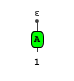
\includegraphics[scale=0.99]{obrazky/sxsx1.png}
}
\qquad
\subfloat[$T(2)$.]{
\label{img:sxsx2}
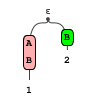
\includegraphics[scale=0.99]{obrazky/sxsx2.png}
}
\qquad
\subfloat[$T(3)$.]{
\label{img:sxsx3}
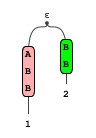
\includegraphics[scale=0.99]{obrazky/sxsx3.png}
}
% \qquad

\subfloat[$T(4)$.]{
\label{img:sxsx4}
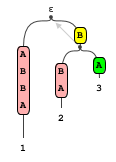
\includegraphics[scale=0.99]{obrazky/sxsx4.png}
}
\qquad
\subfloat[$T$.]{
\label{img:sxsx5}
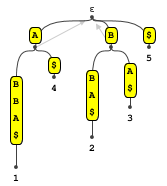
\includegraphics[scale=0.99]{obrazky/sxsx5.png}
}
\caption{\emph{Sufixové stromy.} Na obrázku sú sufixové stromy pre slová 
{\tt A}, {\tt AB}, {\tt ABB}, {\tt ABBA}, {\tt ABBA\uz}. Šípky znázorňujú 
sufixové linky, ružovou a zelenou sú označené hrany, na ktoré sa bude v 
nasledujúcom, kroku aplikovať prvé pravidlo. Čísla oznažujú, na ktorom znaku 
začína daný sufix v slove.}
\label{img:sxsx}
\end{figure}

\subsection{Zhrnutie}

Sufixový strom $T$ pre slovo $w = w_1w_2w_3\cdots w_n\uz$, vytvoríme tak, že z 
prázdneho stromu vytvoríme postupne stromy $T(1), T(2), T(3),\ldots, T(n), T$. 

Strom $T(1)$ vytvoríme triviálne; pridáme koreňu hranu s dvojicou indexov 
$(1, e)$ a nastavíme štartovací vrchol $u_s$ na práve vytvorený vrchol.

Postupne vytvárame strom $T(i)$ zo stromu $T(i-1)$ rozšírením stromu 
$T(i-1)$ o písmenko $w_i$\footnote{Respektíve strom $T$ zo stromu 
$T(n)$ o písmenko $w_n$.} nasledovne:

\begin{enumerate}
\item index $e$ nastavíme na novú hodnotu $i$; 
Tým sme vykonali všetky prvé prípady. Vieme si udržiavať ich počet $j$;
\item za aktuálny vrchol $u$ si zvolíme štartovací vrchol $u_s$;
\item z aktuálneho vrcholu prejdeme po hrane vyššie a zapamätáme si reťazec 
$\alpha$;
\item ak nie sme v koreni, prejdeme po sufixovom linku. Nastavíme aktuálny 
vrchol;
\item z aktuálneho vrcholu vyhľadáme reťazec $w_{j+1}\cdots w_i$;
\item teraz môže nastať druhý alebo tretí prípad:
\begin{itemize}
\item ak nastal druhý prípad, v prípade potreby rozdelíme hranu. Nastavíme 
aktuálny vrchol na posledný navštívený (respektíve vytvorený) a v prípade 
potreby nastavíme sufixový link. K aktívnemu vrcholu pripojíme hranu s 
indexami $(i,e)$, zvýšime index $j$ o 1 a nastavíme štartovací vrchol na 
práve vytvorený. Vrátime sa na krok~3;
\item ak nastal tretí prípad, v prípade potreby nastavíme sufixový link.
\end{itemize}
\item zvýšime hodnotu $i$ o jeden a vrátime sa na krok 1.
\end{enumerate}
 
Takto vybudujeme sufixový strom pre slovo $w$.

\section{Použitie}

Sufixový strom má v stringológií veľa využití
\citep{gusfield}. Najtriviálnejší je algoritmus na zistenie podreťazca v 
slove. Navyše vieme určiť, na ktore pozícií sa podreťazec vyskytuje. Pri 
konštrukcii stromu stačí označovať listy číslami v poradí podľa vytvorenia. 

Sufixový strom pre viacej reťazcov sa nazýva \emph{všeobecný sufixový strom} 
a dá sa zostrojiť miernou úpravou Ukkonenovho algoritmu. Reťazce $v_1, v_2, 
v_3, \ldots, v_n$ spojíme a oddelíme unikátnymi oddelovačmi. Vznikne nám slovo 
$v_1\uz_1v_2\uz_2v_3\uz_3\cdots v_n\uz_n$, z ktorého vieme vybudovať sufixový 
strom. Tento strom sa dá využiť na vyhľadanie najdlhšieho spoločného 
podreťazca. 

\section{Vizualizácia}

Sufixový strom sme vizualizovali podobne ako písmenkový strom, použili sme 
Walkerov algoritmus \citep{walker} so zakrivenými hranami. Sufixové linky 
sme znázornili šedými šípkami. Na rozdiel od písmenkového stromu sa v 
sufixovom strome vyskytujú na hranách reťazce. Tie sme znázornili ako viac 
spojených hrán.

Pri vizualizácií algoritmu oznažujeme hrany, pre ktoré platí prvý prípad, 
ružovou farbou. Hranu, pre ktorú platí prvý prípad a je pridaná ako posledná, 
označujeme zelenou farbou. Z tejto hrany začína "zaujímavejšia" časť 
rozširovania stromu.



\chapter{Popis softvéru}\label{chap:popis}

V predchádzajúcich kapitolách sme si popísali niektoré dátové štruktúry a 
vybrané algoritmy. Hlavnou náplňou je ich vizualizácia. Ako sme povedali v 
úvode, vizualizácia je názorné vykreslenie dátovej štruktúry. Vizualizácia 
algoritmu je znázornenie priebehu algoritmu na dátovej štruktúre. 

\section{Analýza existujúcich riešení}

Softvér vizualizuje dátové štruktúry, algoritmy na nich a popisuje ako 
algoritmy fungujú. Preto sa hodí ako učebná pomôcka pre študentov na 
samoštúdium a pre učiteľov na názorné ukážky pri vyučovaní.

Vizualizované dátové štruktúry sú známe a rozšírenie vizualizácie je veľké, 
preto exituje veľa podobných aplikácií a appletov znázorňujúcich tieto 
dátové štruktúry a algoritmy. Väčšina z nich je na úrovni školských projektov 
a je súkromná. Preto porovnám len tie vizualizácie, ktoré sú vybrané skupinou 
ľudí venujúcej sa vizualizácií algoritmov; skupinou {\tt algoviz.org}. 
Analýza prebehla v máji 2012.

\subsection{Union/Find Algorithm Visualization (union-find)}\label{sec:ufav}
Tento malý applet je súčasťou väčšieho projektu \emph{Virginia Tech Algorithm 
Visualizations}. Applet je implementovaný v programovacom jazyku \Java\ a po
grafickej stránke je veľmi podobný ako zvyšok projektu. Softvér je vydaný pod 
licenciou {\tt GPL}. Vyvíjali ho Cris Kania a Cliff Shaffer počas jesene 2004. 

Je dostupný na: \url{http://research.cs.vt.edu/AVresearch/UF/}.

\subsubsection{Popis}
Applet poskytuje operácie $\union$ a $\find$ na ôsmich, dvanástich, šestnástich 
alebo dvadsiatich vrcholoch. Na obrázku \ref{img:vis:ufav} je obrazovka 
appletu. Môžeme vidieť, že dátová štruktúra je vykreslená vpravo. Použitý je 
jednoduchý algoritmus. Vpravo dole je vykreslená reprezentácia v poli a 
pre každý vrchol je vypísaný otec. Vľavo je riadne vypísaný zoznam vykonaných 
krokov, ktorý je navyše farebne odlíšený. Farby vo výpise a vo vizualizácií 
spolu korešpondujú. Vľavo dole sú nastavenia. 
Applet poskytuje operácie $\union$ s heuristikou na spájanie a $\find$ s 
možnosťami bez kompresie a s kompresiou cesty 
(popísané v sekciách \ref{sec:komp-union} a \ref{sec:komp-cesta}).

\begin{figure}
\centering
\greybox{%
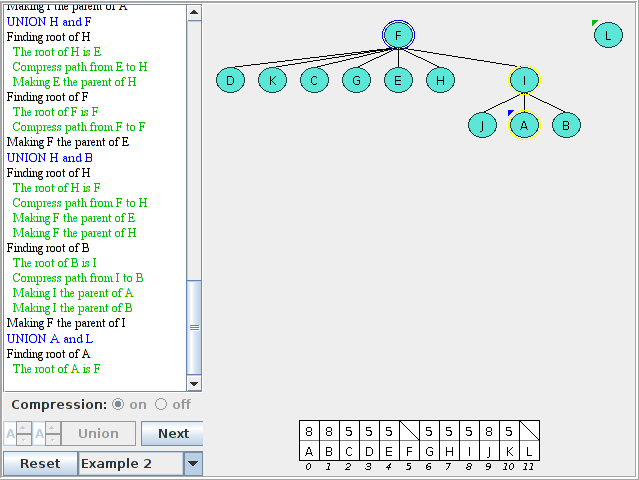
\includegraphics[scale=0.5]{obrazky/union-find-kania-shaffer-fall-2004}%
}
\caption{\emph{Softvér Union/Find Algorithm Visualization.} V ľavej časti 
obrazovky sa nachádzajú výpisy a možnosti nastavenia, vpravo je vizualizácia 
dátovej štruktúry a prebiehajúceho algoritmu.}
\label{img:vis:ufav}
\end{figure}

%\subsection{Hodnotenie}
Softvér poskytuje priestor len na malé príklady. Na 
pochopenie ako fungujú algoritmy to je postačujúce. Ovládanie je intuitívne.

\subsection{AlVie (union-find)}\label{sec:alvie}
% \citat{%
% The girl's name Alvie, also used as boy's name Alvie, is a variant of Alvina 
% (old English), and the meaning of Alvie is "elf or magical being, friend".}{%
% \url{http://alvie.algoritmica.org/alvie3/quickstart}}

AlVie je veľký projekt. Je to prostredie na vizualizáciu algoritmov, 
vytváranie vlastných vizualizácií a veľmi flexibilné pridávanie vlastného 
materiálu. Slúžil na podpru talianských škôl. Projekt momentálne spravuje 
Pilu Crescenzi. Je implementovaný v jazyku \Java.

\subsubsection{Popis}
Na webovej stránke projektu (\url{http://alvie.algoritmica.org/alvie3}) je 
prehľadný popis funkcionality a používania. Aplikácia ponúka množstvo 
nastavení a veľa možností exportovania danej vizualizácie. Avšak nepodarilo sa 
mi nastaviť si vlastný vstup, preto som ostal len pri základnej možnosti. 
Union-find je tu bohužiaľ implementovaný nie cez les, ale ako spájaný zoznam 
(obr. \ref{img:vis:alvie}), čo asymptoticky spomaľuje beh algoritmu.

\begin{figure}
\centering
\greybox{%
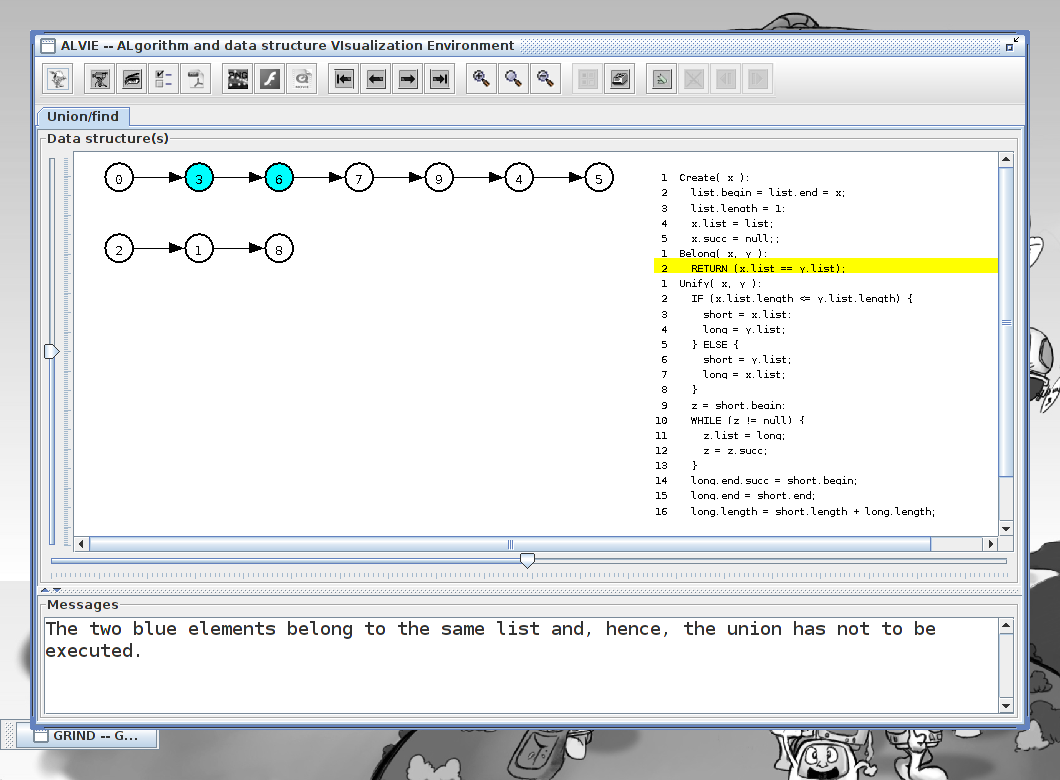
\includegraphics[scale=0.37]{obrazky/AlVie}%
}
\caption{\emph{Softvér Alvie.} Prebieha {\tt XML} skript. Vpravo je pomocný 
pseudokód.}
\label{img:vis:alvie}
\end{figure}

Napriek veľkému množstvu dodávaných algoritmov, nastavení a 
zobrazenému pseudokódu počas vizualizácie má tento softvér nevýhody v podobe 
horšieho ovládania a neoptimálnej implementácie disjunktných množín.

\subsection{Data Structure Visualizations (union-find)}\label{sec:galles}

Vizualizácia union-find algoritmu je v tomto prípade súčasťou veľkého projektu 
využívajúceho veľa technológií (Flash, \Java, {\tt HTML5}). Autorom je David 
Galles.

Projekt je prístupný na: 
\hbox{\url{http://www.cs.usfca.edu/~galles/visualization/}}.

\subsubsection{Popis}

Autor si dal záležať na použití moderných technológií a celá internetová 
aplikácia vyzerá veľmi pekne. Aplikácia zobrazuje štruktúru aj ako les aj ako 
pole. Dá sa nastaviť rýchlosť algoritmu a možnosti heuristík. Vstupné 
parametre operácií sa zadávajú cez textové políčka.

\begin{figure}
\centering
\greybox{%
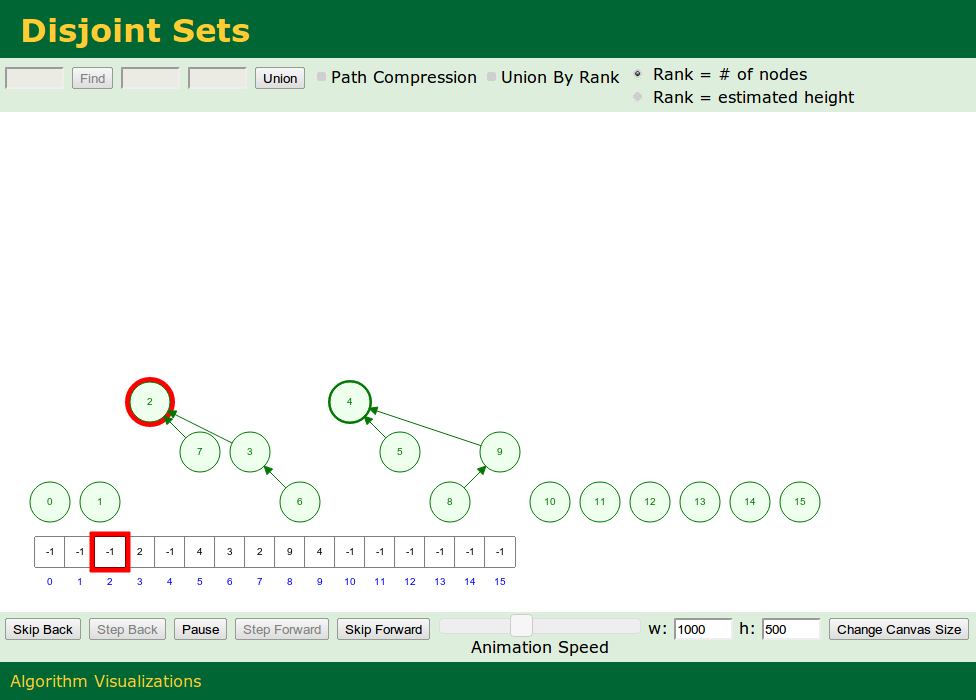
\includegraphics[scale=0.37]{obrazky/galles}%
}
\caption{\emph{Softvér Data Structure Visualizations.} Prebieha spájanie dvoch 
množín. Celá aplikácia beží v internetovom prehliadači.}
\label{img:vis:galles}
\end{figure}

Aplikácia je dobre popísaná, dá sa na nej nastaviť všetko potrebné vrátane 
rýchlosti premietania a veľkosti vykreľovacej plochy. Nevýhodou je, že 
nevypisuje, čo sa práve deje a teda používateľ musí algoritmus poznať.

\subsection{TRAKLA2 (trie)}\label{sec:trakla}

TRAKLA2 je učebná pomôcka vyvíjaná skupinou ľudí "Software visualization 
group". Všetci sú študenti alebo zamestnanci na Helsinskej technickej 
univerzite. Obsahuje veľa algoritmov a ku každému má sadu úloh, ktoré žiak 
môže riešiť. 

Celý výučbový systém je dostupný a popísaný na: 
\url{http://www.cse.hut.fi/en/research/SVG/TRAKLA2/index.shtml}.

\begin{figure}
\centering
\greybox{%
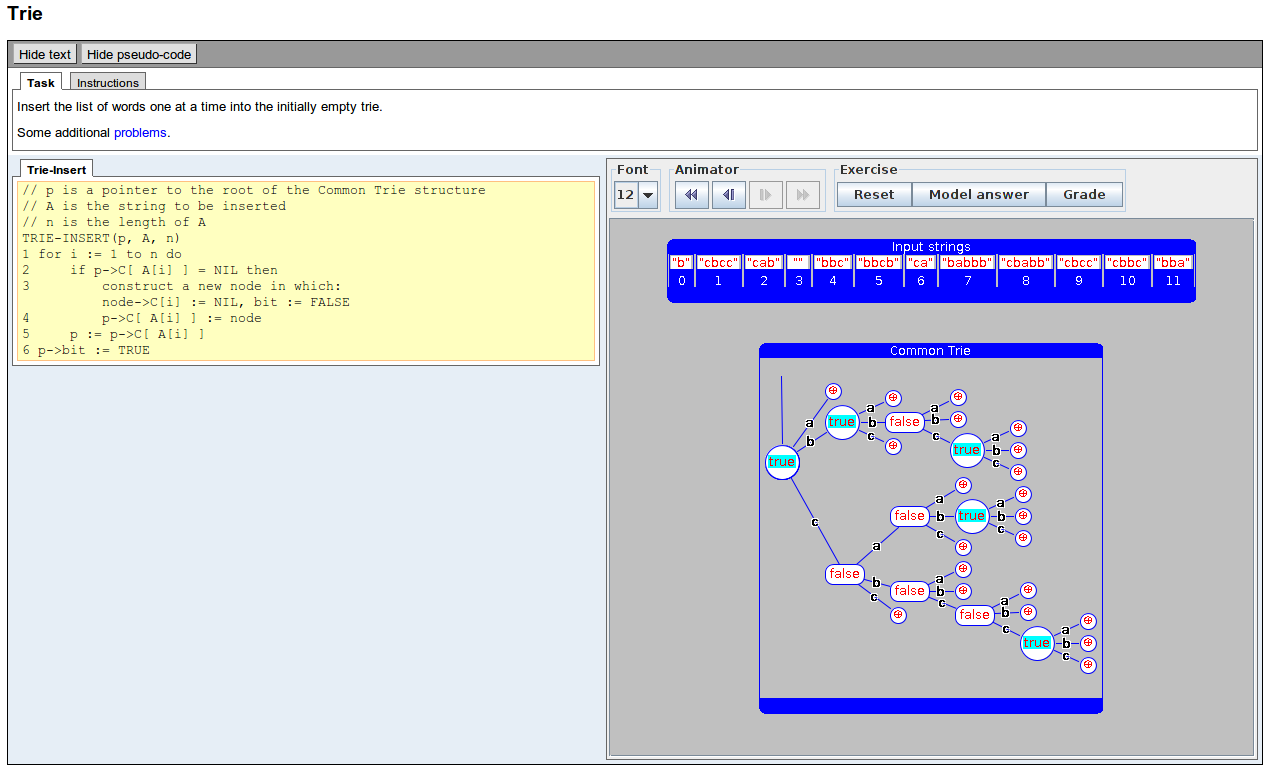
\includegraphics[scale=0.33]{obrazky/trakla2}%
}
\caption{\emph{Prostredie TRAKLA2.} Riešenie zadania; budovanie písmenkového 
stromu obsahujúceho zadané reťazce. Celá aplikácia beží v internetovom 
prehliadači.}
\label{img:vis:trakla2}
\end{figure}

\subsubsection{Popis}

Už na prvý pohľad je vidieť, že na projekte sa podieľa veľa ľudí. Stojí za ním 
viac ako 40 ľudí. Systém je premyslený, každý algoritmus obsahuje pseudokód. 
Všade sú pomôcky, takže ak sme niečomu nerozumeli, našli sme navigáciu na 
odpoveď. 

Samotné vizualizovanie písmenkového stromu je vykonávané niektorým tesným 
algoritmom, čo je veľká výnimka pri vizualizáciach, ktoré sa nezaoberajú tým, 
ako vykresľovať grafy! V hornej časti je umiestnený pomocný text, vľavo je 
pseudokód a vpravo je dátová štruktúra, na ktorej sa vykonáva zadanie (obrázok 
\ref{img:vis:trakla2}). Je možné zvoliť si veľkosť písma.

Všetko je spravené pekne a prehľadne, možno grafická stránka by sa dala 
vylepšiť. Jediná chyba, na ktorú som narazil bola, že pokiaľ som kroky 
nevykonával v správnom poradí, nebola mi uznaná správna odpoveď aj keď 
výsledok správny bol. Toto je ale špecifická chyba len pre písmenkový strom 
(pre iné dátové štruktúry môže poradie pridávania zmeniť reprezentáciu).

\subsection{Sufixové stromy}

Na sufixové stromy, konkrétne Ukkonenov algoritmus, ktorý sme vizualizovali, 
sa podarilo nájsť len jednu a aj to textovú vizualizáciu. 

\subsection{Ďalšie vizualizácie}

Uviedli sme tri softvéry pre union-find a jeden pre písmenkový 
strom. Na jednoduché 
písmenkové stromy sme viac vizualizácií nenašli. Ďalšie programy vizualizovali 
textové dáta alebo iné modifikácie písmenkových stromov (niektoré sú uvedené v 
sekcií \ref{sec:trie:pouzitie}).

Všetky aplikácie, ktoré sme analyzovali, však mali jeden spoločný nedostatok. 
Nedalo sa rýchlo dostať ku stavu, kedy je na štruktúre vykonaných veľa operácií 
a pokračovať z tohto stavu ďalej. Na prázdnej dátovej štruktúre nemusí byť 
dobre vidieť priebeh operácie. Taktiež to môže byť nepríjemné v prípade, že si 
chce používateľ len pripomenúť na už existujúcej štruktúre ako algoritmus 
funguje, prípadne ako štruktúra po vykonaných operáciách vyzerá.
% \todo{
% Cieľom tejto etapy je oboznámenie sa s prostredím, v ktorom bude aplikácia používaná. 
% Dôraz sa kladie na hlbšie pochopenie interakcie aplikácie s prostredím. 
% Ak existujú, treba vykonať aj analýzu podobných systémov.
% }

\clearpage
\section{Špecifikácia požiadaviek}

Počas analýzy sme zistili, že vizualizácie mali nedostatky najmä v tom, že sa 
na nich nedalo naraz vykonať viac operácií. V prípade, že sa dalo (sekcia 
\ref{sec:alvie}), tak sa z tohto stavu nedalo pokračovať. Ďalej sme zistili, 
že aplikácie neposkytujú rozšírené metódy vstupu. Všeobecne bolo veľmi 
obtiažne vôbec vybudovať väčšiu dátovú štruktúru, na ktorej by boli algoritmy 
a hlavne ich efektivita viditeľnejšia. Pri niektorých vizualizáciach nebolo 
jasne viditeľné, čo sa ide vykonať.

\subsection{Požiadavky}

Naša aplikácia bude používaná najmä študentmi, ktorí si chcú zopakovať učivo 
z prednášok, alebo učiteľmi, ktorí túto aplikáciu budú chcieť využívať na 
hodinách.

Preto sa nám zdalo byť vhodné, aby študent dostával výpisy o tom, čo sa bude 
diať a aby bolo prostredie pre študenta dostatočne používateľsky príjmené. Pre 
učiteľa je potrebné, aby sa aplikácia prijateľne zobrazovala cez projektor, 
aby bola dátová štruktúra od začiatku naplnená (veľakrát sa algoritmy 
vysvetlujú na pripravenej dátovej štruktúre) a taktiež, aby bolo prostredie 
používateľsky príjemné.

Softvér ako taký mal vizualizovať tieto veci:
\begin{itemize}
\item dátovú štruktúru pre disjunktné množiny reprezentovanú stromom a na nej 
tieto algoritmy:
	\begin{itemize}
	\item naivné spájanie, spájanie podľa ranku;
	\item nekomprimované hľadanie, hľadanie s jednoduchou kompresiou, hľadanie s 
	delením cesty, hľadanie s pólením cesty.
	\end{itemize}
\item písmenkový strom (trie) a na ňom tieto algoritmy:
	\begin{itemize}
	\item vkladanie slova;
	\item testovanie na prítomnosť slova;
	\item mazanie slova.
	\end{itemize}
\item sufixový strom a jeho vytváranie pomocou Ukkonenovho algoritmu.
\end{itemize}

\subsection{Prevádzkové požiadavky}

Pretože ľudia používajú rôzne operačné systémy a softvér nepracuje so 
špecifickými systémovými zdrojmi bolo potrebné, aby bola aplikácia nezávislá 
od operačného systému. Keďže má byť dostupná na študentské účely, nemala by 
byť hardvérovo náročná.
% \todo{
% Východiskom tejto etapy je etapa analýzy. 
% Zaoberá sa úlohami, ktoré má aplikácia zabezpečiť. 
% Oboznámime sa s prostredím, v ktorom bude aplikácia používaná. 
% Zaujímame sa o to, čo chce zadávateľ riešiť, čo požaduje, aby aplikácia vykonávala a pre koho je určená. 
% Zatiaľ nás nezaujíma spôsob realizácie.  
% Cieľom špecifikácie požiadaviek je stanovenie služieb, ktoré zákazník požaduje od systému a ohraničenia na jeho vývoj a prevádzku. 
% Teda zaujímame sa o funkcionálnu stránku systému, potom o to, aké by mali byť vstupy a výstupy systému 
% a s akými údajmi systém bude pracovať, potom o prevádzkové požiadavky 
% (počet a charakteristika používateľov, časová odozva systému, potrebný hardvér a softvér, bezpečnosť a ochrana systému a iné potrebné požiadavky). 
% Prevádzkové požiadavky nazývame aj nefunkcionálne požiadavky. 
% Detailný opis špecifikácie požiadaviek na softvér  najdeme v (1) alebo v štandarde IEEE 830.
% }

\section{Návrh}

Táto práca je pokračovaním práce Jakuba Kováča a preto návrh vychádzal hlavne z 
jeho práce. Našou hlavnou úlohou bolo implementovať vybrané dátové štruktúry a 
algoritmy. V~nasledujúcich častiach sme popísali požiadavky kladené na náš 
softvér, či už z hľadiska technického alebo používateľského, zvolené 
technológie a rozhranie systému.
% vzťahy medzi časťami softvéru, 
%štruktúru dát a rozhranie systému.

\subsection{Technické požiadavky}

Softvér slúži na vizualizáciu a bolo potrebné ho implementovať multiplatformovo.
Taktiež slúži aj na opisovanie prebiehajúceho algoritmu, teda 
bola potrebná plocha na vykresľovanie, plocha na vypisovanie toho, čo sa deje, 
ovládacie prvky algoritmu a ovládacie prvky na výber dátových štruktúr.

\subsection{Používateľské požiadavky}

Ako sme už naznačili, používateľmi sú prevažne študenti a učitelia, veľmi 
pravdepodobne informatiky. Preto bolo vhodné okrem obyčajného a pomalšieho 
zadávania vstupu po jednej operácií vytvoriť prostredie, v ktorom sa bude dať 
zadávať aj zložitejší vstup.

Ďalej bolo potrebné názorne vizualizovať dátové štruktúry a všetko podstatné k 
pochopeniu algoritmov. Konkrétne pri union-finde išlo o prípadné ranky, 
pri písmenkovom strome o odstraňovanie vetiev, prehľadné vykresľovanie pri 
prebiehajúcich algoritmoch a pri sufixovom strome sufixové linky, práve 
pridávaný sufix a celé slovo, ktorému sufixový strom budujeme.

\subsection{Použité technológie}

Keďže projekt bol pokračovaním predošlej práce za hlavný programovací jazyk 
bola zvolená \Java. Na grafické znázornenie sú to jednotlivé triedy balíkov 
AWT a Swing. Na generovanie náhodných reťazcov sme použili špeciálne upravenú 
triedu s návrhovým vzorom \emph{singleton}. Vďaka celkovej nenáročnosti na 
technológie a zameraniu projektu nebolo potrebné použiť viac technológií.

\subsection{Rozhranie aplikácie}

Rozhranie vizualizácií bolo podobné ako všetkých iných štruktúr 
implementovaných v predošlej verzií softvéru. Vstupné dáta boli zadávané do 
vstupného textového poľa, alebo klikaním myšou. Podľa stlačeného tlačidla sa 
spustil daný proces. Výstupne údaje boli prezentované vo vykresľovacom okne 
pre dátovú štruktúru a vo výpise pre komentáre. Vykreslená štruktúra sa dala 
zväčšiť, zmenšiť a posunúť pomocou myšky.

Pre každú dátovu štruktúru bolo potrebné zabezpečiť vstupné textové pole, 
prípadne dodatočné vstupné metódy a tlačidlá pre všetky operácie.

\subsubsection{Union-find}

Pre union-find bolo potrebné zabezpečiť vstupné textové pole, tlačidlá pre 
operácie $\union$ a $\find$, vyberanie vstupných prvkov myšou, možnosť výberu 
medzi naivným spájaním a spájaním podľa ranku a medzi hľadaním zástupcu bez 
kompresie, s jednoduchou kompresiou, delením cesty a pólením cesty (popísané 
v kapitole \ref{chap:uf}).

\subsubsection{Písmenkový strom}

Pri písmenkovom strome bolo nutné zabezpečiť vstupné pole tak, aby sa do systému 
dostali slová, len s abecedou, ktorú chceme. Pre nás abecedu tvorili veľké 
písmená anglickej abecedy. Ďalej bolo potrebné, aby sa dal pridať do stromu 
ucelenejší text. Na vykonávanie operácií $\put$, $\find$ a $\delete$ bolo 
potrebné implementovať tlačidlá.

\subsubsection{Sufixový strom}

Sufixový strom bolo potrebné vytvoriť zo vstupného slova. Preto treba na tento 
účel implementovať jedno tlačidlo.

\subsection{Prepojenie s predošlým systémom}

Po implementácií mal systém tvoriť jeden celok, preto bola potreba dbať na 
celistvosť a podobný štýl programovania. Na jednotlivé implementovanie 
obrazoviek, vstupných polí a tlačidiel bolo nutné použiť už existujúce 
rozhranie a tak isto na implementáciu vizualizácie bolo treba použiť rovnaký 
systém, ktorý vyžadoval dedenie z predpripravených abstraktných tried. 

V hornej lište aplikácie bolo menu na výber dátových štruktúr a menu 
na výber jazyka. Systém fungoval na princípe kontajnera inštanciovaných tried 
udržiavajúcich jednotlivé obrazovky. Objekty mali priradenú dátovú štruktúru. 
Panel obsahoval plochy pre vykresľovanie, výpis komentárov (toho, čo sa bude 
diať) a ovládacie tlačidlá. Pri vykonaní zvolenej operácie sa spustilo nové 
vlákno vykonávajúce danú operáciu a obsluhujúcu obrazovku.

Všetky predošlé vizualizácie pracovali s binárnymi stromami. Naše dátové 
štruktúry však boli všeobecné stromy, respektíve lesy. Preto bolo nutné 
implementovať triedu na prácu so všeobecnými stromami.
% \todo{
% V tejto etape sa ujasňuje koncepcia systému. 
% Navrhne sa jeho dekompozícia, určia sa vzťahy medzi časťami systému a ohraničenia funkcionality. 
% Túto časť návrhu zvyčajne modelujeme technikami softvérového inžinierstva napr. procesným modelom DFD (Data Flow Diagram, str.24 v (1)) 
% Dekompozícia sa môže urobiť aj na základe iných princípov ako je funkcionálny (str. 53 v (1)). 
% V ďalšom sa identifikuje štruktúra údajov, ktoré do systému vstupujú, ktoré systém spracováva a produkuje. 
% Vzťah medzi údajmi sa modeluje entitno-relačným diagramom, v ktorom sa pomenovávajú vzťahy medzi údajovými entitami. 
% Ak použijeme model DMD (Data Model Diagram), potom v ňom znázorňujeme kvantifikované vzťahy dohodnutými značkami na označenie kardinality. 
% Ak rozložíme vzťah typu M:N pomocou väzobnej entity, potom dostávame fyzický model údajov.  (str.31 v (1))
% V etape návrhu sa navrhne rozhranie systému ( čo do systému vstupuje a čo z neho vystupuje), 
% navrhne sa typ používateľského rozhrania (príkazovo orientované rozhranie, menu, priame riadenie, komunikácia v prirodzenom jazyku ), 
% plán realizácie systému a stanovia sa podmienky, za akých bude používateľ akceptovať produkt. 
% Odhadnú sa potrebné ľudské a materiálne zdroje a navrhne sa postup zaškolovania používateľov.
% }


\chapter{Implementácia softvéru}\label{chap:implementacia}

V tejto kapitole postupne uvedieme realizáciu návrhu popísaného 
v~kapitole~\ref{chap:popis}. Popíšeme ako sme vizualizovali dané 
dátové štruktúry a algoritmy (sekcia \ref{sec:im:vis}) a ukážeme si 
implementáciu a ovládanie aplikácie (sekcia \ref{sec:im:im}). 
Na záver uvedieme ako dopadlo testovanie softvéru (sekcia \ref{sec:im:test}).
% \todo{
% Programovo realizujeme podrobný návrh databázovej aplikácie. 
% Vypracuje sa podrobná dokumentácia k vytvorenému produktu. 
% Vytvorí sa používateľská príručka, kde sa podrobne dokumentuje používateľské rozhranie, spresní sa popis funkcií a spôsob ich aktivácie.
% }

\section{Vizualizácia}\label{sec:im:vis}

Základom pre vizualizáciu dátových štruktúr bol upravený algoritmus pre 
tesné vykresľovanie a použitie rôznych farieb pre prehľadnejšiu vizualizáciu.

\begin{figure}
\centering
\includegraphics[scale=0.63]{obrazky/ufshow}
\caption{\emph{Vizualizácia union-find.} Jednotlivé množiny sú vykresľované 
tesne a sú od seba oddelené pomyselnou zvislou čiarou.}
\label{img:ufshow}
\end{figure}

\subsection{Union-find}

Dátovú štruktúru union-find sme vizualizovali ako les. Pre názorné 
oddelenie množín sme si zvolili pravidlo, ktoré zakazovalo vykresliť vrchol 
z iného stromu (prvok inej množiny) 
napravo od najľavejšieho vrcholu a naľavo od napravejšieho vrcholu inej 
množiny. Jednotlivé množiny sme už vykreslovali tesným Walkerovým algoritmom 
\citep{walker}. Vykresľovanie je znázornené na obrázku~\ref{img:ufshow}.

Vizualizácia poskytuje všetky heuristiky na spájanie a 
nájdenie reprezentanta množiny a 
aj tlačidlo na vykonanie viacerých náhodných spojení naraz. Toto je užitočné, 
keď chce používateľ vidieť, ako dátová štruktúra vyzerá, po vykonaní 
veľkého počtu operácií. Okrem bežného textového vstupu je možné vyberať prvky aj myšou. 
Vybrané prvky sú zvýraznené.

\subsubsection{Operácia $\find$}

Hľadanie reprezentanta množiny sme vizualizovali tak, že sme vybratý prvok 
označili, vyznačili sme cestu do koreňa a reprezentanta množiny 
(algoritmus dopredu nepozná reprezentanta, ale v rámci vizualizácie sme to 
považovali za vhodné). Následne sme vykonali kompresiu, aktívny vrchol je 
modrý. Cestu sme nechali 
znázornenú šedou farbou, aby bolo vidieť, ako vyzerá cesta pred a po prevedení 
algoritmu. 

Pre heuristiky delenie a pólenie cesty sme použili ružovú farbu na označenie 
syna a vnuka, keďže tieto algoritmy s nimi pracujú. Operácia $\find$ je 
znázornená na obrázku~\ref{img:kompresia}.

\subsubsection{Operácia $\union$}

Spájanie prvkov sme vizualizovali vykonaním dvoch hľadaní reprezentanta a 
následného napojenia reprezentantov podľa typu algoritmu.

\begin{figure}
\centering
\includegraphics[scale=0.80]{obrazky/trie}
\caption{\emph{Vizualizácia písmenkového stromu.} Písmenkový strom obsahuje 
slová {\tt ADAM\uz, HODIL\uz, JAGAVU\uz, JAHODU\uz, JASNE\uz, K\uz, MAGDE\uz, 
MALUJUCEJ\uz, POKRAJANU\uz, POLOVICU\uz, POMARANCA\uz, S\uz, TRPKYMI\uz, 
VYSNAMI\uz}.}
\label{img:trieshow}
\end{figure}


\subsection{Písmenkový strom}

Pri vizualizácií písmenkového stromu sme použili 
Walkerov algoritmus pre úsporné rozloženie vrcholov v strome
\citep{walker}. Keď má vrchol viacej synov a hrany kreslíme priamo, tak vzniká 
nedostatok priestoru pre umiestnenie znakov na hrany. Preto sme sa rozhodli 
kresliť hrany zakrivene, podľa Bézierovej krivky. 
Vo vizualizácií sa dajú vložiť náhodné slová podľa momentálne nastaveného 
jazyka. Taktiež sa automaticky odstraňuje diakritika a interpunkcia, takže 
sa dá naraz vložiť súvislý text (obrázok~\ref{img:trieshow}).

\subsubsection{Operácia $\trieinsert$}

Aby bolo zreteľné, aké slovo vkladáme, znázorňujeme zbytok vkladaného slova 
pri mieste, kde sa práve v strome nachádzame. Časť, ktorú sme vložili a aj 
časť, ktorú ideme vložiť vypisujeme bielou na modrom pozadí. Miesto, na ktoré 
sa presunieme, prípadne kam ideme pripájať, sme označili ružovou farbou. 
Ukončovací znak (\uz) sme vykresľovali tmavšie a menším písmom.

\begin{figure}
\centering
\includegraphics[scale=0.55]{obrazky/treexfind}
\caption{\emph{Hľadanie slova {\tt MORE\uz}.} Ružovou je vyznačené hľadané 
slovo. Šedou je označená množina písmen, na ktoré sa algoritmus práve 
pozerá.}
\label{img:triefind}
\end{figure}

\subsubsection{Operácia $\find$}

Podobne ako pri vkladaní slova, aj pri vizualizácií hľadania slova, sme 
použili pomocnú bublinu so zbytkom nespracovaného vstupu. Na rozdiel od 
vkladania sme použili ružovú farbu. Na znázornenie množiny prvkov, kde sa môže 
vyskytovať následujúce písmenko sme použili šedú farbu 
(obrázok~\ref{img:triefind}).

\subsubsection{Operácia $\delete$}

Mazanie slova z písmenkového stromu sme implementovali ako nájdenie slova a 
následné zmazanie prípadnej mŕtvej vetvy (popísané v sekcii 
\ref{sec:trie:popis}). Na nájdenie slova sme použili ten istý farebný princíp, 
ako pri operácií $\find$. Mŕtvu vetvu sme zvýraznili červenou farbou 
(obrázok~\ref{img:triedelete}).

\subsection{Sufixový strom}

Sufixový strom sme vizualizovali podobne ako písmenkový strom, použili sme 
Walkerov algoritmus \citep{walker} so zakrivenými hranami. Sufixové linky 
sme znázornili šedými šípkami. Na rozdiel od písmenkového stromu sa v 
sufixovom strome vyskytujú na hranách reťazce. Tie sme znázornili ako viac 
spojených hrán a text sme spojili.

\subsubsection{Ukkonenov algoritmus}

Pri vizualizácií algoritmu (obrázok~\ref{img:sxsx}) označujeme hrany, pre 
ktoré platí prvý prípad, 
ružovou farbou. Hranu, pre ktorú platí prvý prípad a je pridaná ako posledná, 
označujeme zelenou farbou. Z tejto hrany začína "zaujímavejšia" časť 
rozširovania stromu. Pri pridávaní sufixov do stromu sme použili modrú farbu.

\begin{figure}
\centering
\greybox{\includegraphics[scale=0.4]{obrazky/guigui}}
\caption{\emph{Grafické rozhranie softvéru Gnarley Trees.} V hornej časti je 
lišta s menu pre výber dátových štruktúr a voľbu jazyka. Hlavnú časť 
obrazovky tvorí priestor na vykresľovanie dátových štruktúr. Vpravo je 
priestor na popis udalostí. Dole sú ovládacie tlačidlá.}
\label{img:gui}
\end{figure}

\newpage
\section{Popis ovládania}\label{sec:im:im}

Obrazovka softvéru sa skladá z menu na výber dátových štruktúr, menu na výber 
jazyk, obrazovky na vykresľovanie, ovládacích tlačidiel a obrazovky na výpis 
komentárov (obrázok~\ref{img:gui}).

Keď si z menu vyberieme dátovú štruktúru zobrazí sa inicializovaná dátová 
štruktúra a príslušné tlačidlá. Celá dátová štruktúra sa dá posúvať ťahaním 
myšou, približovať alebo odďaľovať použitím kolieska myši, alebo automaticky 
vystrediť a priblížiť pomocou tlačidla.

\subsection{Union-find}

\paragraph{Vstup.} Vstup zadávame do vstupného poľa alebo vyberieme prvok 
myšou. Prioritu majú prvky vybrané myšou. Pre operáciu $\find$ sa vyberie prvý 
prvok, pre operáciu $\union$ sa vyberú prvé dva prvky. Pokiaľ je zadaný menší 
počet prvkov náhodne sa doplnia. 

\paragraph{Náhodné spojenie.} Tlačidlo pre vykonanie viacerých náhodných 
spojení berie parameter -- počet spojení zo vstupného poľa. Pokiaľ nie je 
hodnota zadaná, za parameter sa berie základná hodnota.

\subsection{Písmenkový a sufixový strom}

\paragraph{Vstup.} Do vstupného poľa zadávame slová oddelené medzerou. Textový 
vstup sa pred pridávaním ošetrí: odstráni sa diakritika, interpunkcia a čísla. 
Následne sa text prevedie na veľké písmená a za každé slovo sa pridá 
ukončovací znak (\uz). Prázdne slovo sa do stromu dá pridať zadaním vstupného 
reťazca "\uz". Pokiaľ je vstup prázdny, vykoná sa pridanie náhodného slova 
podľa nastaveného jazyka.

\paragraph{Náhodné vloženie.} Tlačidlo pre vykonanie viacerých náhodných 
pridaní funguje ako pri algoritme union-find. Slová, ktoré pridá, sú vybraté 
z~databázy slov nastaveného jazyka. Sufixový strom sa vytvára pre jedno 
slovo, a preto nemá zmysel pridávať viacero náhodných slov.


\section{Testovanie, prevádzka a údržba}\label{sec:im:test}

Pri testovaní aplikácie sa nevyskytli nečakané chyby. Za najväčšie nedostatky 
sme považovali občas nezrozumiteľné komentáre a neoptimálne znázornenie 
Ukkonenovho algoritmu. Pri premietaní cez projektor sme prišli na nedostatok: 
niektoré farby sú príliš sýte, a preto sa kontrast medzi písmom a pozadím zdá 
byť malý a farby príliš tmavé. Tento problém sa vyskytoval len občas, ale 
pri bežnom osvetlení.

Softvér nepotrebuje špecifickú údržbu, keďže sa jedná o samostatnú aplikáciu. 
Avšak vhodné je sledovať aktualizácie, ktoré opravujú chyby. Vývoj a aj 
najnovšie verzie sú voľne dostupné na systéme pre správu zdrojových kódov 
Github, konkrétne na webovej stránke: \url{https://github.com/kuk0/alg-vis}. 
Stabilná verzia s popisom algoritmov sa nachádza na stránke: 
\url{http://people.ksp.sk/~kuko/gnarley-trees}. Na oboch sídlach sa nachádzajú 
kontakty, ktorými môže používateľ upozorniť na chyby v aplikácií.
% \todo{
% Testovanie sa vykonáva v prevádzkovom prostredí zvyčajne u používateľa. 
% Vykonávame testovanie jednotlivých  dekomponovaných častí a chovanie aplikácie ako celku. 
% Overujeme, či vytvorený produkt zodpovedá špecifikácii a spľňa požiadavky používateľa
% }

% \todo{
% Prevádzku má na starosti používateľ, ktorý sleduje situácie pri ktorých vznikli chyby. 
% Ďalší rozvoj systému a opravy sleduje jeho tvorca - dodávateľ.
% } 


\backmatter
\cleardoublepage
\phantomsection
\addcontentsline{toc}{chapter}{Záver}
\chapter*{Záver}\label{chap:outro}
Tu by malo byť niečo v zmysle, že som to strašne nestihol a vymenované všetko, čo by som chcel dorobiť?

\backmatter

\cleardoublepage
\phantomsection
\addcontentsline{toc}{chapter}{Literatúra}
% http://en.wikipedia.org/wiki/BibTeX
% http://sites.stat.psu.edu/~surajit/present/bib.htm
% \bibliographystyle{plain}
% \bibliographystyle{alpha}
% \bibliographystyle{apalike}
% \bibliography{literatura}

\printbibliography


\end{document}

